
% RetailSec AI Presentation
% Theme: Metropolis (Modern, Clean, Professional)

\documentclass[aspectratio=169]{beamer}

% Theme selection
\usetheme[numbering=fraction, progressbar=frametitle]{metropolis}
\usecolortheme{default}

% Packages
\usepackage{graphicx}
\usepackage{booktabs}
\usepackage{tikz}
\usetikzlibrary{positioning, arrows.meta, shapes.geometric}
\usepackage{pgfplots}
\pgfplotsset{compat=1.18}

% Metadata
\title{RetailSec AI}
\subtitle{Next-Gen Autonomous Threat Intelligence for Digital Retail}
\date{}
\author{MUHAMMAD ASLAM A}
\institute{Ideathon 2026}

% Custom Colors (White Background, Black Text)
\definecolor{RetailBackground}{HTML}{FFFFFF} % White
\definecolor{RetailForeground}{HTML}{000000} % Black

\setbeamercolor{background canvas}{bg=RetailBackground}
\setbeamercolor{normal text}{fg=RetailForeground}
\setbeamercolor{frametitle}{bg=RetailBackground, fg=RetailForeground}
\setbeamercolor{title}{fg=RetailForeground}
\setbeamercolor{subtitle}{fg=RetailForeground}
\setbeamercolor{itemize item}{fg=RetailForeground}
\setbeamercolor{itemize subitem}{fg=RetailForeground}
\setbeamercolor{enumerate item}{fg=RetailForeground}

% Force standout frame to be white/black
\setbeamercolor{palette primary}{bg=RetailBackground, fg=RetailForeground}

% Improve Spacing
\setbeamertemplate{itemize/enumerate body begin}{\setlength{\itemsep}{1.5em}}
\setbeamertemplate{itemize/enumerate subbody begin}{\setlength{\itemsep}{1em}}

% Override number to be X / 12
\setbeamertemplate{frame numbering}{
  \insertframenumber{} / 12
}

\begin{document}

% Slide 1: Title
\begin{frame}
  \titlepage
\end{frame}

% Slide 2: The Problem
\begin{frame}{The Problem: Retail is Under Attack}
    \textbf{"Cybercriminals are Targeting Your Checkout"}
    \vspace{0.5cm}
    \begin{itemize}
        \item \textbf{Peak Traffic Risks}: malicious bots hide within Black Friday surges.
        \item \textbf{Loyalty Fraud}: Attackers drain points and gift cards from high-value accounts.
        \item \textbf{Silent Breaches}: Average detection time is \textbf{200+ days}. Retailers lose brand trust instantly.
        \item \textbf{Analyst Burnout}: Security teams drown in false positives during sales events.
    \end{itemize}
\end{frame}

% Slide 3: Threat Landscape
\begin{frame}{Retail-Specific Threats}
    \textbf{Beyond Standard Attacks}
    \vspace{0.5cm}
    \begin{enumerate}
        \item \textbf{Gift Card Cracking}: Brute-forcing card numbers to steal balances.
        \item \textbf{Inventory Hoarding}: Scalper bots buying up limited stock (PS5/Sneakers).
        \item \textbf{Account Takeover (ATO)}: Using stolen credentials to order goods.
        \item \textbf{Price Scraping}: Competitor bots aggressively scraping pricing data.
    \end{enumerate}
\end{frame}

% Slide 4: Our Solution
\begin{frame}{Proposed Solution: RetailSec AI}
    \textbf{An AI Analyst that Understands Commerce}
    \vspace{0.2cm}
    We build a specialized intelligence layer that distinguishes between a \textit{loyal customer} and a \textit{sophisticated bot}.
    \vspace{0.3cm}
    \begin{description}
        \item[Context Aware] Knows that 50 logins/min is normal for a sale, but abnormal for a single user.
        \item[Generative Explanation] \textbf{Llama-3} explains: \textit{"Blocking user for hoarding inventory during flash sale."}
        \item[Instant Defense] Blocks IP addresses at the edge before inventory is lost.
    \end{description}
\end{frame}

% Slide 5: Architecture
\begin{frame}{System Architecture}
    \textbf{Powered by Modern Tech Stack}
    \vspace{0.5cm}
    \begin{itemize}
        \item \textbf{Frontend}: Next.js 14 (App Router) + Tailwind CSS v4.
        \item \textbf{Validation}: Zod for runtime type safety on log ingestion.
        \item \textbf{Visualization}: Recharts for interactive threat velocity graphs.
        \item \textbf{AI Core}: Groq SDK integration for sub-second LLM inference.
        \item \textbf{Storage}: LocalStorage persistence for session-based analysis.
    \end{itemize}
\end{frame}

% Slide 6: Process Flow
\begin{frame}{Process Flow}
    \centering
    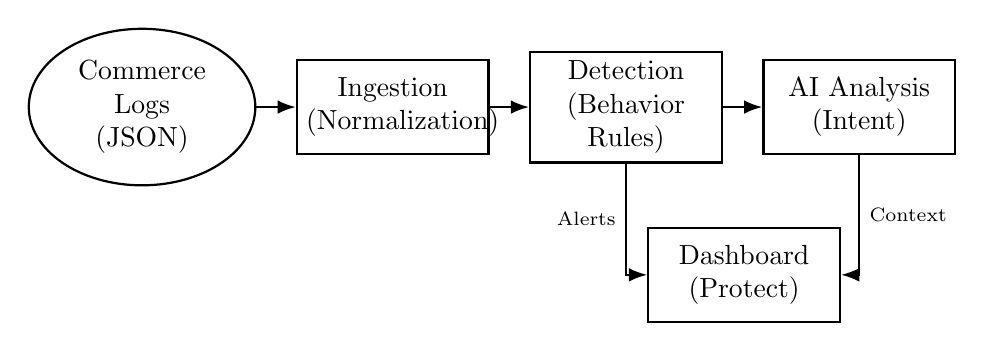
\begin{tikzpicture}[
        node distance=0.8cm and 0.5cm,
        block/.style={rectangle, draw=black, thick, fill=white, text width=2.2cm, align=center, minimum height=1.2cm},
        cloud/.style={ellipse, draw=black, thick, fill=white, text width=1.8cm, align=center},
        arrow/.style={->, >=Latex, thick}
    ]
        % Nodes
        \node[cloud] (logs) {Commerce Logs\\(JSON)};
        \node[block, right=of logs] (ingest) {Ingestion\\(Normalization)};
        \node[block, right=of ingest] (detect) {Detection\\(Behavior Rules)};
        \node[block, right=of detect] (ai) {AI Analysis\\(Intent)};
        
        \node[block, below=of detect, xshift=1.5cm] (dash) {Dashboard\\(Protect)};

        % Paths
        \draw[arrow] (logs) -- (ingest);
        \draw[arrow] (ingest) -- (detect);
        \draw[arrow] (detect) -- (ai);
        \draw[arrow] (detect) |- node[near start, left, font=\scriptsize] {Alerts} (dash);
        \draw[arrow] (ai) |- node[near start, right, font=\scriptsize] {Context} (dash);
    \end{tikzpicture}
\end{frame}

% Slide 7: Dashboard Preview (New)
\begin{frame}{Live Dashboard Preview}
    \centering
    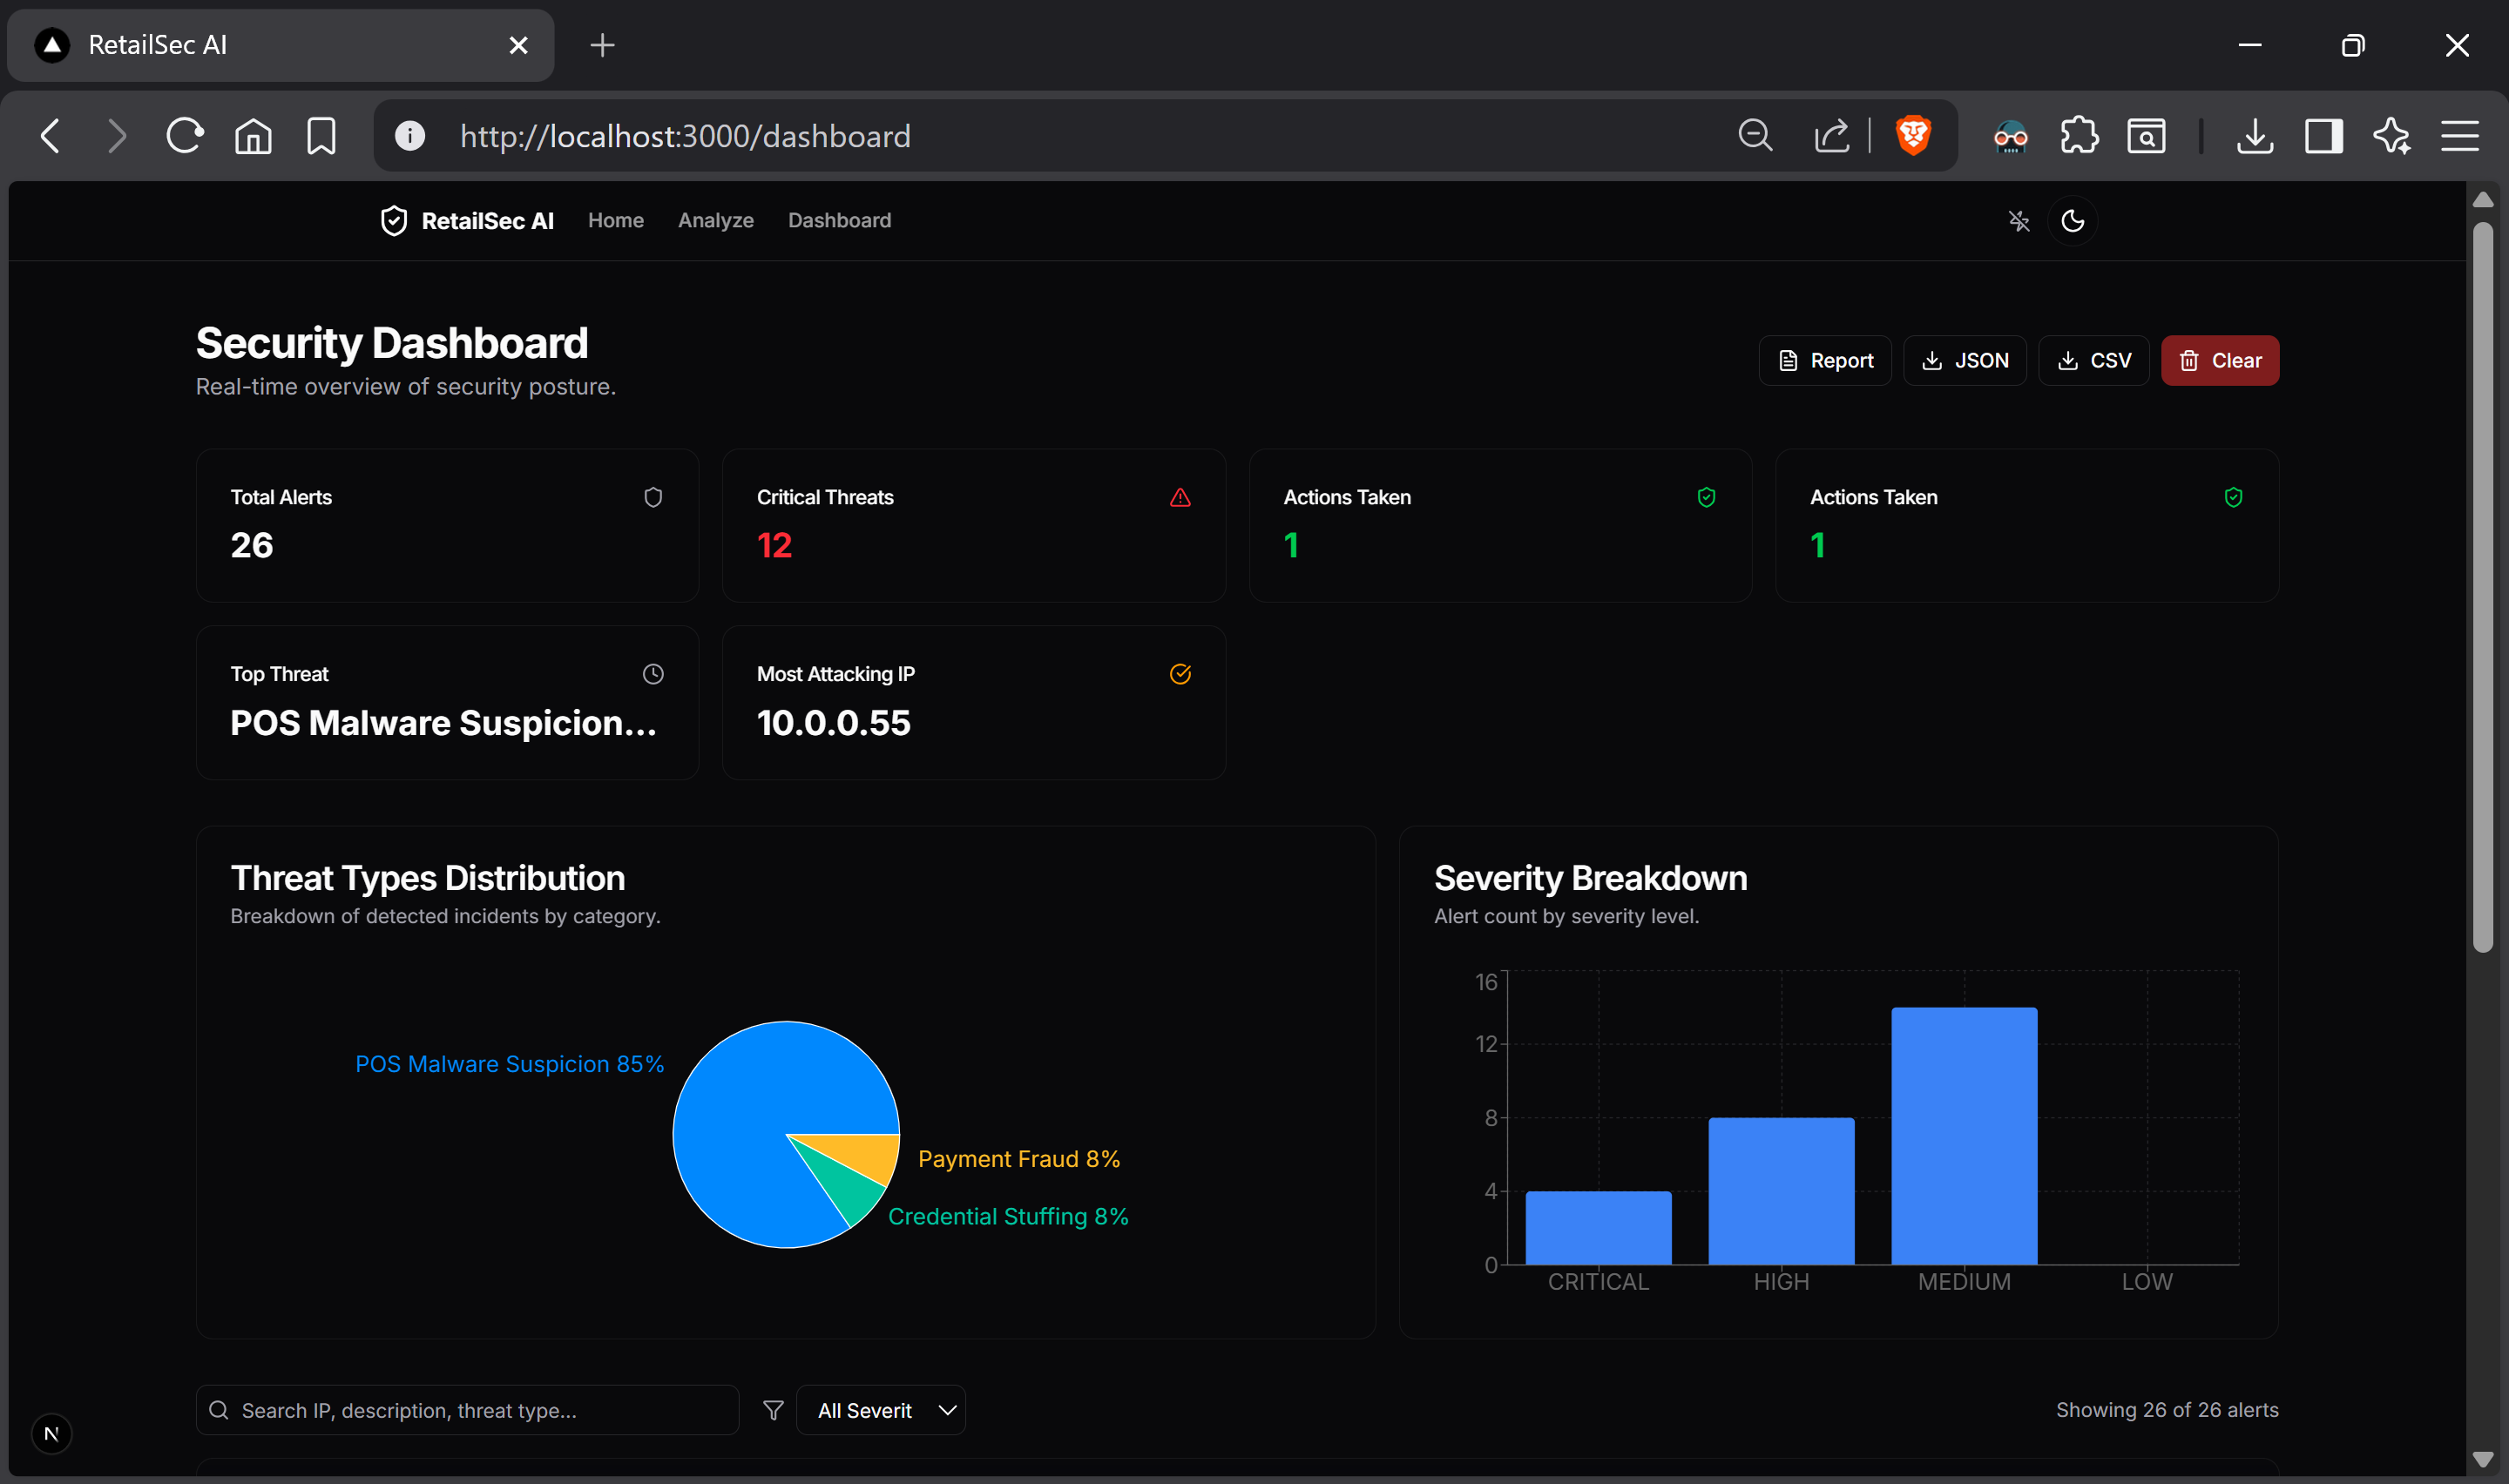
\includegraphics[width=0.48\textwidth]{ss1.png} \hfill
    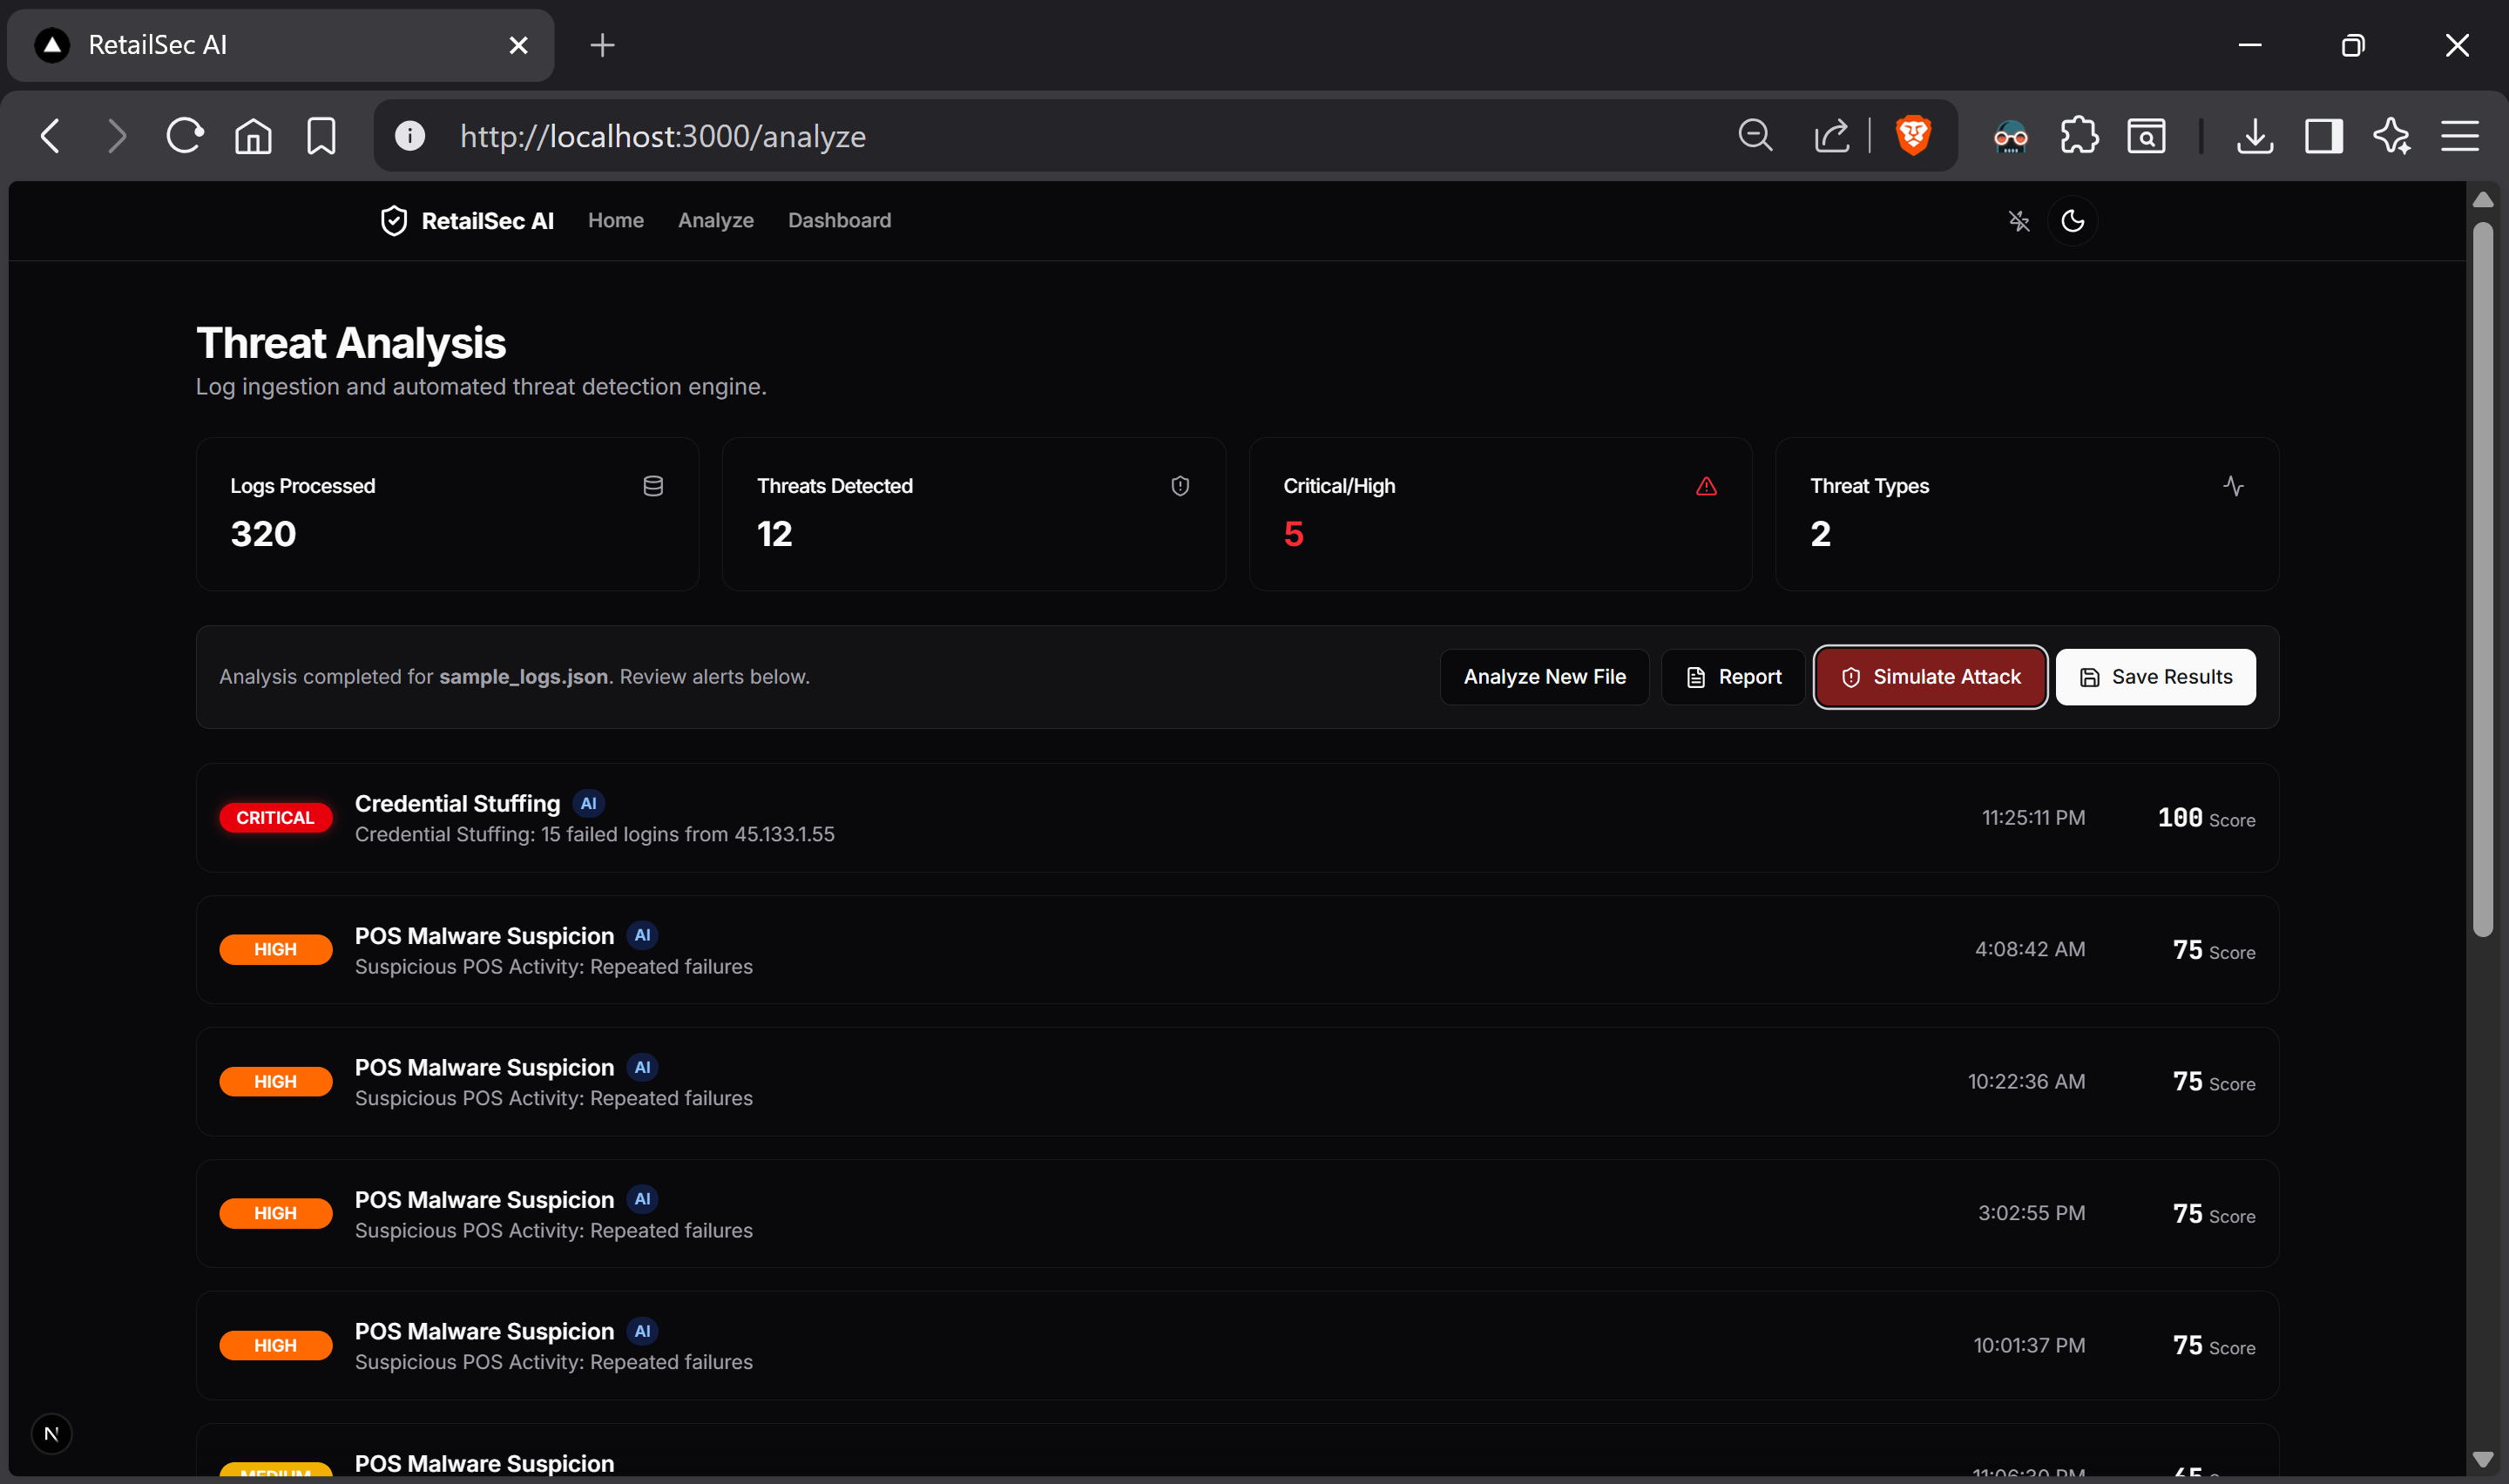
\includegraphics[width=0.48\textwidth]{ss2.png}
    \vspace{0.2cm}
    \begin{itemize}
        \item \small Left: Security Dashboard \hfill Right: Threat Analysis
    \end{itemize}
\end{frame}

% Slide 8: Competitive Edge (New)
\begin{frame}{Why RetailSec AI is Different}
    \textbf{Competitive Edge}
    \vspace{0.5cm}
    \begin{itemize}
        \item \textbf{Retail-Specific Modeling}: Trained on commerce threats (Gift Cards, Inventory), not just generic WAF rules.
        \item \textbf{GenAI Explanations}: Llama-3 explains \textit{why} a block happened, reducing analyst fatigue.
        \item \textbf{One-Click Response}: Instant remediation directly from the dashboard.
        \item \textbf{Lightweight}: Runs on Vercel Edge (Next.js), no heavy SIEM infrastructure required.
    \end{itemize}
\end{frame}

% Slide 7: Demo Walkthrough
\begin{frame}{Demo Walkthrough}
    \textbf{"Stopping a Loyalty Hack"}
    \vspace{0.5cm}
    \begin{enumerate}
        \item \textbf{Ingest}: Upload \texttt{checkout\_logs.json}.
        \item \textbf{Analyze}: System flags "High-Velocity Gift Card Checks".
        \item \textbf{Explain}: \textbf{AI Agent} analyzes behavior:\\ \textit{"User checking 100+ gift cards with 0 purchases. Pattern matches 'Card Cracking'."}
        \item \textbf{Respond}: One-click "Block IP" prevents financial loss.
    \end{enumerate}
\end{frame}

% Slide 8: Impact
\begin{frame}{Impact \& Benefits}
    \begin{columns}
        \column{0.5\textwidth}
        \begin{itemize}
            \item \textbf{Revenue Protection}\\ Stops inventory loss and chargebacks.
            \item \textbf{Customer Trust}\\ Ensures real humans get the products, not bots.
        \end{itemize}
        
        \column{0.5\textwidth}
        \begin{itemize}
            \item \textbf{Operational Efficiency}\\ AI reduces triage time by 90\%.
            \item \textbf{Cost Efficient}\\ Open-source AI (Llama-3) is cheaper than fraud losses.
        \end{itemize}
    \end{columns}
\end{frame}

% Slide 9: Future Scope
\begin{frame}{Future Scope: Roadmap to Production}
    \begin{itemize}
        \item \textbf{Live Streams}: Integrate Apache Kafka during Black Friday.
        \item \textbf{Auto-Remediation}: Webhooks to update Cloudflare WAF / AWS Shield.
        \item \textbf{Federated Learning}: Share fraud patterns with other retailers securely.
        \item \textbf{Voice Interface}: "Hey RetailSec, did we lose any inventory to bots today?"
    \end{itemize}
\end{frame}



\begin{frame}
    \centering
    \Huge\bfseries Thank You!\\
    \large Questions?
\end{frame}

\end{document}
